%%%%%%%%%%%%%%%%%%%%%%%%%%%%%%%%%%%%%%%%%
% Formal Text-Rich Title Page 
% LaTeX Template
% Version 1.0 (27/12/12)
%
% This template has been downloaded from:
% http://www.LaTeXTemplates.com
%
% Original author:
% Peter Wilson (herries.press@earthlink.net)
%
% License:
% CC BY-NC-SA 3.0 (http://creativecommons.org/licenses/by-nc-sa/3.0/)
% 
% Instructions for using this template:
% This title page compiles as is. If you wish to include this title page in 
% another document, you will need to copy everything before 
% \begin{document} into the preamble of your document. The title page is
% then included using \titleGP within your document.
%
%%%%%%%%%%%%%%%%%%%%%%%%%%%%%%%%%%%%%%%%%

%----------------------------------------------------------------------------------------
%	PACKAGES AND OTHER DOCUMENT CONFIGURATIONS
%----------------------------------------------------------------------------------------

\documentclass{book}
\usepackage{graphicx}
\usepackage{dirtytalk}
\usepackage{fancyhdr}
\usepackage{wrapfig}
\usepackage[normalem]{ulem}
\usepackage[utf8]{inputenc}

\pagestyle{fancy}
\fancyhead[LE,RO]{}
\fancyhead[RE,LO]{\rightmark}
\fancyfoot[CE,CO]{\leftmark}
\fancyfoot[LE,RO]{\thepage}

\renewcommand{\headrulewidth}{2pt}
\renewcommand{\footrulewidth}{1pt}




\newcommand*{\plogo}{\fbox{$\mathcal{VTX}$}} % Generic publisher logo

%----------------------------------------------------------------------------------------
%	TITLE PAGE
%----------------------------------------------------------------------------------------

\newcommand*{\titleGP}{\begingroup % Create the command for including the title page in the document
\centering % Center all text
%\vspace*{\baselineskip} % White space at the top of the page

\rule{\textwidth}{1.6pt}\vspace*{-\baselineskip}\vspace*{2pt} % Thick horizontal line
\rule{\textwidth}{0.4pt}\\[\baselineskip] % Thin horizontal line

 {\Huge ARS RHETORICA}\\ {\Large COMPILED FOR \\[0.3\baselineskip] THE NEW SAT (ESSAY)}\\[0.2\baselineskip] % Title

\rule{\textwidth}{0.4pt}\vspace*{-\baselineskip}\vspace{3.2pt} % Thin horizontal line
\rule{\textwidth}{1.6pt}\\[\baselineskip] % Thick horizontal line

\scshape % Small caps-0
A number of fascinating and life-changing explanations and examples \\ % Tagline(s) or further description
presented  in a clear and useable way \\[\baselineskip] % Tagline(s) or further description

\vspace*{1\baselineskip} % Whitespace between location/year and editors

Written by \\[\baselineskip]
{\Large ZENG FAN PU\par} % Editor list
{\itshape Hwa Chong Institution \\ Singapore\par} % Editor affiliation

\vspace*{\baselineskip} % Whitespace between location/year and editors
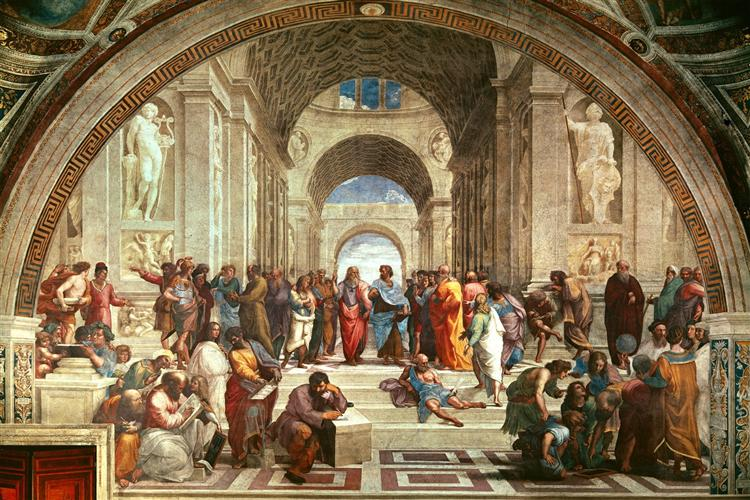
\includegraphics[scale=0.6]{SchoolOfAthens}

\vfill % Whitespace between editor names and publisher logo

\plogo \\[0.3\baselineskip] % Publisher logo
{\scshape 2016} \\[0.3\baselineskip] % Year published
{\large VORTEX PUBLISHINGS}\par % Publisher

\endgroup}

%----------------------------------------------------------------------------------------
%	BLANK DOCUMENT
%----------------------------------------------------------------------------------------

\begin{document} 
\thispagestyle{empty}
%\pagestyle{empty} % Removes page numbers

\titleGP % This command includes the title page
\pagenumbering{arabic}
\setcounter{tocdepth}{4}

\tableofcontents
\chapter{Rhetoric}
\section{Overview}

\begin{itemize}
	\item Set your \textbf{goals} and the argument's \textbf{tense}
	\item Think of whether you want to emphasize \textbf{character}, \textbf{logic}, or \textbf{emotion}
	\item Make sure the \textbf{time} and the \textbf{medium} are ripe for persuasion
\end{itemize}

\textbf{Cicero's speech outline:}
\begin{enumerate}
	\item Introduction
	\item Narration
	\item Division
	\item Proof
	\item Refutation
	\item Conclusion
\end{enumerate}

\section{Goals}
\subsection{Personal Goal}
What you want from your audience
\subsection{Audience Goals}
\begin{itemize}
	\item Mood: This is the easiest thing to change
	\item Mind: A step up in difficulty from changing the mood
	\item Willingness to act: Hardest of all, because it requires an emotional commitment and identification with the action 
\end{itemize}

\subsection{Issue control} 
Mastering argument's chief topics
\begin{itemize}
	\item Blame (Forensic): Covers the past. Its chief topics are \emph{guilt} and \emph{innocence}
	\item Values (Demonstrative): Get argued in the present tense. Chief topics are \emph{praise} and \emph{blame}.
	\item Choice (Deliberative): Deals with the future. Its chief topic is the \emph{advantageous} - what's best for the audience.
\end{itemize}

\section{Ethos}
This is argument by character - using your reputation or someone else's as the basis for argument. When you give a speech, play up your character - or what you want the audience to think it is. Its three chief aspects are virtue (areté), practical wisdom (phronesis), and disinterest (eunoia).\\

\subsection{Decorum}
Your ability to fit in with the audience's expectation of a trustworthy leader.
\begin{itemize}
	\item Code Grooming: Using language unique to the audience
	\item Identity Strategy: Getting an audience to identify with an action - to see the choice as one that helps define them as a group
	\item Irony: Saying one thing to outsiders with a meaning revealed only to your group
\end{itemize}

\subsection{Virtue, or Cause}
The appearance of living up to your audience's values, areté.
\begin{itemize}
	\item Bragging: The straightforward, and least effective, way to enhance your virtue
	\item Witness Bragging: An endorsement by a third party, the more disinterested the better
	\item Tactical Flaw: A defect or mistake, intentionally revealed, that shows your rhetorical virtue
	\item Switching Sides: Appearing to have supported the powers that be all along
	\item Throwing the support behind the inevitable: Enthusiastically endorse the opponent's view to show off your virtue. Only use if you're bound to lose anyway.
	\item Logic-free Values: Focusing on the individual values-words and commonplaces to bring a group together and get it to identify with you.
	\item Identity: Get people to describe themselves. Usually the first thing they mention reveals their best sense of who they are. And most people will do just about anything to live up to that identity.
	\item The Halo: Sum up the issue in a few words. Suss out the values of your audience. Now, find a representative or piece of the issue that can symbolize those values.
\end{itemize}

\subsection{Practical Wisdom, or Craft}
Phronesis, a type of wisdom relevant to practical things, requiring an ability to discern how or why to act virtuously and encourage practical virtue, excellence of character, in others.

\begin{itemize}
	\item Showing off experience
	\item Bending the rules
	\item Appearing to take the middle course
\end{itemize}

\subsection{Disinterest, or Caring}
Eunoia - an apparent willingness to sacrifice your own interests for the greater good.
\begin{itemize}
	\item Reluctant Conclusion: Appearing to have reached your conclusion only because of its overwhelming rightness
	\item Personal Sacrifice: Claiming that the choice will help your audience more than it will help you.
	\item Dubitatio: Seeming doubtful of your own rhetorical skill
\end{itemize}

\subsection{Liar detector}
Techniques for judging a person's credibility.
\begin{itemize}
	\item Needs Test: Do the persuader's needs match your needs?
	\item Comparable Experience: Has the persuader actually done what he's talking about?
	\item Dodged Question: Ask who benefits from the choice. If you don't get a straight answer, don't trust that person's disinterest.
	\item `That depends' Filter: Instead of a one-size-fits-all choice, the persuader offers a solution tailored to you.
	\item `Sussing' Ability: The persuade cuts to the chase of an issue.
	\item Extremes: How does the persuader describe the opposing argument? How close is his middle-of-the-road to yours?
	\item Extremist Detector: An extremist will describe a moderate choice as extreme.
	\item Virtue Yardstick: Does the persuader find the sweet spot between the extremes of your values?
	\item Code Inoculation: Be aware of the terms that define the groups you belong to, anmd watch out when a persuader uses them.
\end{itemize}

\subsection{Screw-up Recovery}
Enhancing your ethos through your own mistakes.
\begin{itemize}
	\item Set your goals right after you screw up
	\item Be first with the news
	\item Switch immediately to the future
	\item Avoid belittling the victim
	\item Don't apologize. Instead, express your feelings about not living up to your standards.
\end{itemize}

\section{Pathos}
Argument by emotion is the seductive part of persuasion. Pathos can cause a mood change, make an audience more receptive to your logic, and give them an emotional commitment to your goal.

\subsection{Sympathy}
Registering concern for your audience's emotions.
\begin{itemize}
	\item Oversympathizing: Exaggerated sympathy can make your audience feel ashamed of an emotion you want to change.
\end{itemize}

\subsection{Belief}
This is the key to emotion.
\begin{itemize}
	\item Experience: Refer to the audience's own experience, or plant one in their heads; this is the past tense of belief.
	\item Storytelling: A way to give the audience a virtual experience.
	\item Expectation: Make an audience expect something good or bad, and the appropriate emotion will follow.
\end{itemize}

\subsection{Volume Control}
Underplaying an emotion, or gradually increasing it so that the audience can feel it along with you
\begin{itemize}
	\item Simple speech: Don't use fancy language when you get emotional.
\end{itemize}

\subsection{Unannounced Emotion}
Avoid tipping off your audience in advance of a mood. They'll resist it.

\subsection{Passive Voice}
If you want to direct an audience's anger away from someone, imply that the action happened on its own: ``The chair got broken,'' not ``Pablo broke the chair.''

\subsection{Backfire}
You can calm an individual's emotion in advance by overplaying it yourself. This works especially well when you screw up and want to prevent the wrath of an authority.

\subsection{Persuasive Emotions}
\begin{itemize}
	\item Anger: One of the most effective ways to rouse an aud ience to action. But it's a short-lived emotion.
	\item Belittlement Charge: Show your opponent disrespecting your audience's desires. A belittled audience is an angry one.
	\item Patriotism: Attaches a choice or action to the audience's sense of group identity.
	\item Emulation: Emotional response to a role model. The greater your ethos, the more the audience will imitate you.
	\item Humor: A good calming device that can enhance your ethos.
		\begin{itemize}
			\item Urbane Humor: Plays off a word or part of speech.
			\item Wit: Situational Humor.
			\item Facetious Humor: Joke telling, a relatively ineffective form of persuasion.
			\item Banter: Snappy answers - works best in defense.
		\end{itemize}
\end{itemize}

\subsection{Figures of Speech}
\begin{itemize}
	\item Cliché Twisting: Using overworked language to your advantage.
		\begin{itemize}
			\item Literal Interpretation: Reducing a cliché to absurdity by seeming to take it at face value.
			\item Surprise Ending: Starting a cliché as it's normally said, but ending it differently.
			\item Reworking: Switching words around in a cliché
		\end{itemize}
	\item Word Swap: Changing normal usage and grammar for effect.
		\begin{itemize}
			\item Chiasmus: Creates a crisscross sentence.
		\end{itemize}
	\item Weighing both sides: Comparing or contrasting opinions in order to define the issue.
		\begin{itemize}
			\item Either/Or Figure (Dialysis): Weighs each side equally.
			
			\textit{``You're either for us, or against us.''}
			\item Contrasting Figure (Antithesis): Emphasizes the difference between the two ideas.
			
			\textit{``The success of our economy has always depended not just on the size of our gross domestic product, but on the reach of our prosperity...'' (Barack Obama)}
			\item Meaning-change Figure (Antistasis): Repeats a word in a way that uses or defines it differently. 
			
			\textit{``He that composes himself is wiser than he that composes a book." (Benjamin Franklin)}
		\end{itemize}
	\item Editing Out Loud: Interrupting yourself or your opponent to correct something.
		\begin{itemize}
			\item Self-correction Figure (Metanoia): Lets you amplify an argument while seeming to be fair and accurate.
			\item Redefiner (Correctio): Repeats the opponent's language and corrects it.
		\end{itemize}
	\item Volume Control: Amplifying or calming speech through figures.
		\begin{itemize}
			\item Ironic understatement. 
			
			\textit{``I lived at West Egg, the — well, the less fashionable of the two, though this is a most superficial tag to express the bizarre and not a little sinister contrast between them.'' (The Great Gatsby by F. Scott Fitzgerald)}
			\item Climax: Uses overlapping words in successive phrases in a rhetorical crescendo.
			\texttt{...the author lays example after example of (positive/negative events), building }
			
		\end{itemize}
	\item Word Invention: Figures help you create new words or meanings from old words
		\begin{itemize}
			\item Verbing (Anthimeria): Turns a noun into a verb or vice versa.
			\item ``Like'' Figure (Parelcon): Strips a word of meaning and uses it as a pause or for emphasis. \emph{(``Like,'' ``You know,'')}
		\end{itemize}
\end{itemize}

\section{Logos}
Argument by logic. People like to think that all argument should be nothing but logic; however, Aristotle said that when it comes to persuasion, rational speech needs emotion and character as well.

\subsection{Deduction}
Applying a general principle to a particular matter.

\begin{itemize}
	\item Enthymeme: A logic sandwich that contains deduction. ``We should [choice], becuase [commonplace].'' Aristotle took formal logic's syllogism, stripped it down, and based it on a commonplace instead of a universal truth.
	\item Proof Spotter: A proof consists of examples or a premise. A premise usually begins with ``because,'' or implies it.
	\item Commonplace: Any cliche, belief, or value that can serve as your audience's boiled-down public opinion. It's the starting point of your argument.
		\begin{itemize}
			\item Babbling: An audience's repetition of a word or idea; it often reveals a commonplace.
			\item Rejection: Another good commonplace spotter. An audience will often use a commonplace when it rejects your argument.
			\item Commonplace Label: Applying a commonplace to an idea, a proposal, or a piece of legislation as part of a definition strategy.
		\end{itemize}
\end{itemize}

\subsection{Induction}
Argument by example. It starts with the specific and moves to the general. 

\begin{itemize}
	\item Fact, Comparison, Story: The three kinds of examples to use in inductive logic.
\end{itemize}

\subsection{Concession}
Using your opponent's own argument to your advantage.

\subsection{Framing}
Shaping the bounds of an argument. 

\begin{itemize}
	\item Framing Strategy
		\begin{enumerate}
			\item Find the audience's commonplaces.
			\item Define the issue broadly, appealing to the values of the widest audience.
			\item Deal with the specific problem or choice, using the future tense.
		\end{enumerate}
	\item Definition Strategy: Controlling the language used in an argument.
	\item Term Change: Inserting your own language in place of your opponent's.
	\item Redefinition: Accepting your opponent's terms while changing their connotation.
	\item Definition Jujitsu: Using your opponent's language to attack him.
	\item Definition Judo: Using terms that contrast with your opponent's, creating a context that makes him look bad.
\end{itemize}

\subsection{Logical Fallacies}
\begin{itemize}
	\item Bad Proof: The argument's commonplace or principle is unacceptable, or the examples are bad.
	\begin{itemize}
			\item False Comparison: Two things are similar, so they must be the same.
			\item Fallacy of Association: A is a member of group B. A is a member of group C. Therefore, group B is C. For example, natural ingredients are good for you, so anything called ``natural'' is healthful.
			\item Appeal to Popularity (Argumentum ad populum): Concludes that a proposition is true because many or most people believe it: ``If many believe so, it is so.''
			\item Hasty Generalization: Uses too few examples and interprets them too broadly
			\item Misinterpreting the Evidence: Takes the exception and claims it proves the rule.
			\item Unit Fallacy: Confusing the part for the whole
			\item Argument from Ignorance (Ad Ignorantium): Claims that if something has not been proven, it must be false.	
	\end{itemize}

	\item Bad Conclusion: We're given too many choices, or not enough, or the conclusion is irrelevant to the argument.
		\begin{itemize}
			\item Many Questions: Squashes two or more issues into a single one. Committed when someone asks a question that presupposes something that has not been proven or accepted by all the people involved.
			\item False Dilemma: Offers the audience two choices when more actually exist.
			\item Fallacy of Antecedent: If P, then Q. Therefore, not P, then not Q.
			\item Red Herring: Introduces an irrelevant issue to distract or confuse the audience. Eg. \emph{``There is a lot of commotion regarding saving the environment. We cannot make this world an Eden. What will happen if it does become Eden? Adam and Eve got bored there!''}
			\item Straw Man: Sets up a different issue that's easier to argue. Eg. \emph{``Obama's going to take all our guns!''}
		\end{itemize}
	\item Disconnect Between Proof and Conclusion: The proof stands up all right, but it fails to lead to the conclusion.
		\begin{itemize}
			\item Tautology: A logical redundancy; the proof and the conclusion are the same thing
			\item Reductio ad Absurdum: Takes the opponent's choice and reduces it to an absurdity
			\item Slippery Slope: Predicts a series of dire events stemming from one choice.
			\item Post Hoc Ergo Propter Hoc: Assumes that if one thing follows another, the first thing caused the second one.
		\end{itemize}
\end{itemize}

\subsection{Rhetorical Fouls}
Mistakes or intentional offenses that stop an argument dead or make it fail to reach a consensus.
\begin{itemize}
	\item Switching Tenses Away From The Future: It's fine to use the past or present, but deliberative argument depends on eventually discussing the future.
	\item Inflexible Insistence On The Rules: Using the voice of God, sticking to your guns, refusing to hear the other side
	\item Humiliation: An argument that sets out only to debase someone, not to make a choice
	\item Innuendo: A form of irony used to debase someone. It often plants an idea in the audience's head by denying it.
	\item Threatening (Argumentum ad Baculum): It denies the audience a choice.
	\item Nasty Language or Signs
	\item Utter Stupidity
\end{itemize}

\section{Kairos}
The Romans called it occasio, the art of seizing the occasion. Kairos depends on timing and the medium.

\subsection{Persuadable Moment}
When the audience is ripest for your argument
\begin{itemize}
	\item Moment Spotter: Uncertain moods and beliefs - when minds are already beginning to change - signal a persuadable moment.
	\item Perfect Audience: Receptive, attentive, and well disposed toward you
	\item Audience Change: If the current audience isn't ready for persuasion, seek another one. This is what market research is all about.
\end{itemize}

\subsection{Senses}
The five senses are key to the proper medium.
\begin{itemize}
	\item Sight: Mostly pathos and ethos
	\item Sound: The most logical sense
	\item Smell, Taste and Touch: Almost purely emotional
\end{itemize}

\section{Speechmaking}
\subsection{Invention}
The crafting part of a speech. Its tools are the tools of logos.

\subsection{Arrangement}
The organization of a speech. Ethos first, then logos, then pathos.
\begin{itemize}
	\item Introduction (Exordium): The ethos part, which wins you the interest and the good will of the audience. 
	\item Narration, or Statement of Facts: Tell the history of the matter or list your facts and figures. If you have time, do both. This part should be brief, clear, and plausible. Don't repeat yourself. State the facts in chronological order, but don't begin at the beginning of time - just the part that is relevant to the immediate argument. Don't startle the audience with ``believe it or not'' facts - this part should be predictable. What they hear should sound usual, expected, and natural.
	\item Division: List the points where you and your opponent agree and where you disagree. This is where you can get into definitions as well. It's a biologial issue. It's an ethical issue. It's a rights issue. It's a practical issue (what benefits our society the most?). It's a fairness issue. Division can actually help your ethos, if you use the reluctant conclusion.
	\item Proof: Here is where you get into your actual argument, setting out your argument packet (``We should do this because of that'') and your examples.
	\item Refutation: Destroy your opponent's (anticipated) arguments here.
	\item Conclusion: Restate your best points and, if you want, get a little emotional.
\end{itemize}

\subsection{Style}
Choice of words that make a speech attractive to the listener. The five virtues of style:
\begin{itemize}
	\item Proper Language: Use words that suit the occasion and your audience
	\item Clarity: Would the least informed reader understand it?
	\item Vividness (Enargeia): The ability to create a rhetorical reality before the audience's very eyes. Involves all five senses.
	\item Decorum: The art of fitting in. Behave the way your audience expects you to.
	\item Ornament: Rhythm of your voice and the cleverness of your words. Does it sound good when you read it aloud?
\end{itemize}
	
\subsection{Memory}
The ability to speak without notes.

\subsection{Delivery}
The action of giving a speech.
\begin{itemize}
	\item Voice: Should be loud enough for the room
	\item Gesture: The eyes are key, even in a large room, because they lead your other facial muscles. Use few hand gestures in a formal speech.
\end{itemize}


\end{document}